% ---
% Capitulo de METODOLOGIA
% ---


\chapter{Metodologia}\label{cap:metodologia}
Nesta seção apresenta-se os materiais e métodos utilizados no desenvolvimento do trabalho proposto.
\section{Materiais e Métodos}

% Reescrever
O presente estudo classifica-se como uma pesquisa experimental, em que os experimentos foram realizados
para avaliar o desempenho do Sistema de tempo real Zephyr\cite{Zephyr}
versão 1.14 no microcontrolador ESP32-WROOM-32D de 32 Bits, dois cores e 240MHz, em fatores como analise
de interrupções, sincronização e compartilhamento de recursos e passagem de mensagem
entre outras tarefas mais voltadas para o contexto da missão de um cubesat como alocação em memoria flash.

Foi escolhido o sistema \cite{Zephyr} como alternativa, pois o
mesmo tende a ser um dos mais promissores a ser competitivos perante o FreeRTOS, o benchmark usado é
baseado nos critérios propostos e chamados de benchmarks refinados em \cite{Garcia}, mas também se baseia
na metodologia mais moderna realizada por \cite{Raymundo} no qual apresenta um trabalho muito similar e
completo, mas focado em tecnologias para internet das coisas. Com o objetivo de avaliar se o \cite{Zephyr}
tem qualidade perante a ao FreeRTOS, outro sistema operacional de tempo real mais popular na industria de
cubesats de codigo aberto.

A pesquisa experimental segundo \cite{wazlawick2017metodologia} condiciona o pesquisador a lidar com
diversas variáveis experimentais e variáveis observacionais, visando levar possivelmente, correlações
e dependencias entre as elas, utilizando de técnicas de amostragem e testes de hipóteses.
O mesmo diz que trabalhos desenvolvidos em cima de abordagens padronizadas e
aceitas internacionalmente, apresentando dados empíricos é relevantes, se encaixam no nível mais maduro
de pesquisa, onde o autor deverá apresentar os resultados usando métricas aceitas pela
comunidade, através de observações e medições, implicando que o pesquisador provocará alterações sistemáticas
no ambiente do experimento para se observar os resultados após cada intervenção produzida.

% Questão
% O zephyr rtos tem qualidade perante a outros rtos do 
% mercado na plataforma ESP32?

\section{Configuração do ambiente}


A Figura~\ref{fig: ESP-IDF Software} mostra as principais fases para construir uma aplicação em 
ESP32, abaixo em ESP-IDF encontra-se as bibliotecas e códigos fontes para operar a segunda camada, 
chamada de Toolchain, contem todas as ferramentas para compilação de código que através de ferramentas 
de compilação de projeto externas como CMake e Ninja controem a aplicação final.

\begin{figure}[H]
	\centering
	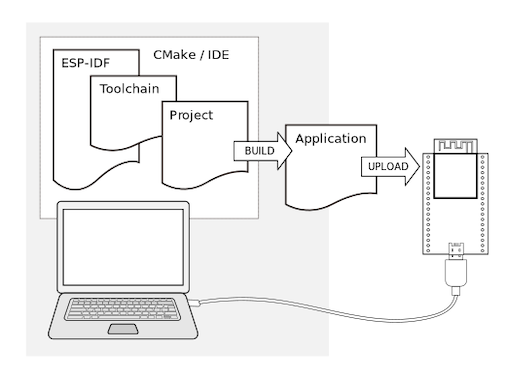
\includegraphics[width=15cm]{imagens/what-you-need.png}
	\caption{Diagrama do processo de construção de uma aplicação para ESP32.}
	Fonte: Retirado de ESP-IDF Programming Guide em https://docs.espressif.com/projects/esp-idf/en/latest/esp32/get-started/index.html
	\label{fig: ESP-IDF Software}
\end{figure}

Todo esse ambiente foi motado na IDE Visual Studio Code, utilizando o plugin PlataformIO para 
desenvolvimento em dispositivos embarcados. A instalação do Zephyr requer diversos passos, para 
facilitar esse processo foi desenvolvido um script de instalação na linguagem Shell Script, o mesmo 
foi disponibilizado no site github em 
\footnote{https://gist.github.com/talesmm14/148b9e02966b038f9334dcbbc4c5451a} para consulta.


% 1 Descrição do objetivo do estudo
% 2 Delineamento da pesquisa
%\subsection{Implementação dos métodos}

%\subsection{Métricas}
\section{Critérios de avaliação}
Segundo \cite{Garcia} existe uma necessidade de avaliação de desempenho de
sistemas de computador em tempo real, pois os mesmos devem operar em
períodos de tempos determinísticos em aplicações críticas. Diante disto
realizaremos os seguintes testes de performance.

\subsection{Velocidade de troca entre tarefas}
Uma tarefa de prioridade mais alta permanece dormente, em quanto a segunda tarefa
com prioridade inferior desperta a primeira tarefa, o tempo de mudança entre as
tarefas e medido.

%Algoritmo Soma Ponderada
\begin{algorithm}
	\SetAlgoLined
	\Entrada{Problema de Teste \textit{FTest}, Número de variáveis de decisão \textit{Nvar}, Número de iterações \textit{Niter}, limites inferiores e superiores das variáveis de decisão \textit{LB,LU}}
		% Parâmetros para as restrições de desigualdade e igualdade \textit{A, Aeq, b,beq} } 
		\Saida{Vetor de soluções ótimas \textit{Svec}}
		\Inicio{
			$ Svec \leftarrow vector(Niter) $; \tcc*[f]{Cria vetor de Soluções} \\
			$ x0 \leftarrow \textsc{rand}(Nvar,1);  $ \tcc*[f]{Cria vetor com Nvar variáveis} \\
			\Para{i  de 1 até Niter }{
				$ W \leftarrow \textsc{Weights(FTest)}; $ \tcc*[f]{Cria vetor de pesos} \\
				$ Fobj \leftarrow \textsc{WeightedSum(Ftest, W)} ; $\tcc*[f]{Transforma a função} \\
				$Svec[i] \leftarrow \textsc{fmincon}(Fobj,x0,A,b,Aeq,beq,LB,LU);$ \tcc*[f]{Encontra e armazena a solução ótima} \\
			}
			%$plot(Svec);$ \tcc*[f]{Imprime gráfico das soluções} \\
		}
		\Retorna{$Svec$}
		\label{algo:soma-ponderada}
		\caption{\textsc{Método da Soma Ponderada}}
	\end{algorithm}

	% \begin{lstlisting}[caption={Classe controladora de Grupos},label={example}]
	% 	class GruposController extends ApiService { 
	% 	  Future<List<Grupos>> listGroups() async { // Get lista de grupos
	% 		List responseList = await get("grupos");
	% 		var parse = responseList;
	% 		List<Grupos> grupos = parse.map((json) => Grupos.fromJson(json)).toList();
	% 		return grupos;
	% 	  }
	% 	  Future<Grupos> GroupAnalytcs(idGrupo) async { // Post de grupo passando id
	% 		var status;
	% 		var prefs = await SharedPreferences.getInstance();
	% 		var url = "dadosgrupo/";
	% 		Map id = {"idGrupo": idGrupo};
	% 		var response = await post(url, id);
	% 		Map mapResponse = json.decode(response.body);
	% 		if (response.statusCode == 200) {
	% 		  status = Grupos.fromJsonPost(mapResponse);
	% 		  prefs.setString("status", mapResponse["status"]);
	% 		} else {
	% 		  status = null;
	% 		}
	% 		return status;
	% 	  }
	% 	}
		
	% 	\end{lstlisting}

\subsection{Tempo de passagem de mensagens entre tarefas}
Uma tarefa será responsável por enviar as mensagens para uma fila vazia, outra
tarefa ira receber a mensagem, o tempo de envio e recebimento das mensagens e
medido.

\begin{figure}[H]
	\centering
	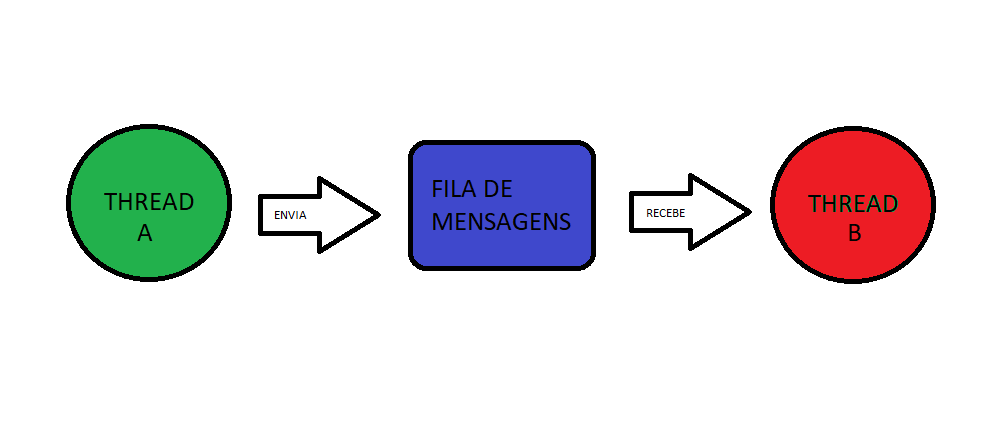
\includegraphics[width=15cm]{imagens/fila_mensagens.png}
	\caption{A tarefa A envia uma mensagem, a tarefa B recebe.}
	Fonte: Autoria Própria.
	\label{fig: fila_mensagens}
\end{figure}

Uma tarefa de prioridade maior solicita uma mensagem de uma fila vazia, uma tarefa
de prioridade menor enviar a mensagem, o tempo de solicitação e envio de mensagem e
medido.

\subsection{Tempo de bloqueio e liberação de desbloqueio de Semáforo e Mutex}
Uma tarefa solicita e libera em seguinte um semáforo, o tempo de bloqueio e
liberação do semáforo são medidos, o mesmo teste e realizado com um Mutex.

\begin{figure}[H]
	\centering
	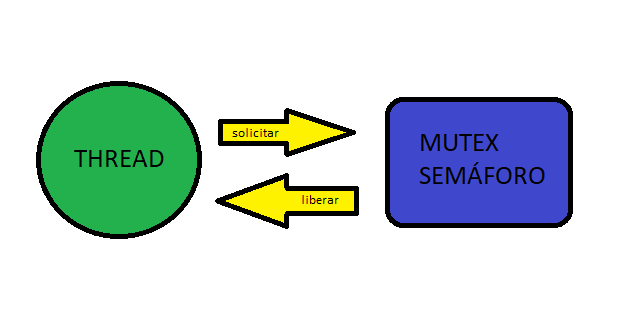
\includegraphics[width=15cm]{imagens/solicitar_bloquear.png}
	\caption{A tarefa solicita e libera uma variável de controle.}
	Fonte: Autoria Própria.
	\label{fig: tempo_semaforo_mutex}
\end{figure}

Uma tarefa de prioridade mais alta solicita o semáforo já bloqueado por uma
tarefa de prioridade inferior, o tempo em que ocorre a mudança entre as tarefas
é medido, o mesmo teste e realizado com um Mutex.

\subsection{Tempo de resposta a eventos externos atraves de interrupção}
Nesse teste será medido o tempo de latência de despacho de uma rotina de serviço de interrupção (ISR) 
e o tempo de despacho de uma tarefa desbloqueada por uma interrupção gerada por um estimulo
externo.

\subsection{Velocidade de alocação de memoria}
Uma tarefa realiza a alocação de espaço na memoria de tamanho fixo de acordo com
as especificações do microcontrolador ESP32, em seguida liberando a memoria,
o tempo de alocação e desbloqueio de memoria são medidos.

\subsection{Velocidade de leitura e gravação em memoria flash (Cartão SD)}
Uma tarefa adquire uma região de espaço na memoria flash disponivel, a mesma gravará
uma quantidade de dados especifica e liberar esta região da memoria, o tempo de adquirir
o espaço, gravar os dados e liberar a memoria serão medidas.


\subsection{Configuração de hardware}
%Aqui serão apresentados os equipamentos utilizados para a elaboração desta pesquisa.

\begin{table}[]
	\centering
	\begin{tabular}{|l|l|}
		\hline
		\textbf{EQUIPAMENTO}                                            & \textbf{UNIDADE} \\
		\hline
		\textcolor[rgb]{0.125,0.129,0.141}{ESP32-DevKitC ESP-WROOM-32U} & 1                \\
		\hline
		\textcolor[rgb]{0.059,0.067,0.067}{Cabo USB-Micro USB}          & 1                \\
		\hline
		Protoboard 400 pontos                                           & 1                \\
		\hline
	\end{tabular}
	\caption{Equipamentos utilizados}
\end{table}

O Hardware escolhido para realizar este estudo foi o ESP32 por possuir varias caracteristicas 
interessantes para uma missão espacial, como temperatura de trabalho de -40° á +85° C, por 
ter dois nucleos e 32-bit, suas configurações de memoria são muito atraentes com 448 KBytes de 
memoria ROM, 520 KBytes de RAM e 4MB de memoria Flash, possui também diversas portas 
GPIO com funções de PWM, I2C, SPI, etc e por ultimo um baixo consumo de corrente de 80mA típica 
e 500mA máxima. Este equipamento foi escolhido por ser de custo baixo, muito utilizado em projetos 
de pequenos satelites e de documentação de facil acesso além de ser compatível com a IDE do Arduino 
permitindo uma simples adoção por toda a comunidade.



\subsection{Medida de tempo}

Para a realização deste benchmark destaca-se a preocupação com a metodologia usada para medir o tempo 
de cada experimento, assim de acordo com a fabricante \cite{} {Expressif} os temporizadores de hardware apresentam 
vantagens em relação aos mesmos implementados em software, um exemplo disto seria que o \cite{FreeRTOS} 
forneçe temporizadores com algumas limitações como a resolução máxima de é igual ao período de ticks 
do próprio sistema operacional, outra limitação está no retorno da chamada do temporizador que são entregues 
por uma tarefa de baixa prioridade, no qual pode conflitar com outras tarefas do sistema. 



